\documentclass{ctexbeamer}        

\usefonttheme{serif}              
\usefonttheme{professionalfonts}  
\usepackage{graphicx}
\usepackage{listings}
\usepackage{mathtools}
\usepackage{hyperref}

\usepackage{url}
\usepackage{tikz}
\usepackage{amsmath}
\usepackage[style=gb7714-2015]{biblatex}
\usepackage{subfigure}
\usepackage{gnuplot-lua-tikz}
\usepackage{float}
\usepackage{xcolor}
\hypersetup{pdfpagemode=FullScreen}  

\usetheme{Frankfurt}       
\usecolortheme{orchid}     


\begin{document}
\lstset{
 columns=fixed,       
 numbers=left,                                            
 commentstyle=\it\color[RGB]{96,6,96},              
 stringstyle=\rmfamily\slshape\color[RGB]{0,128,0},   
}

\title{Julia集的分析和探索}
\author{王麟}
\institute{浙江大学}
\date{2022~年~7~月~4~日}
\frame{\titlepage}



\begin{frame}{目录} 
\begin{center}        
  \tableofcontents[hideallsubsections]
  \end{center}
\end{frame}



\section{引言}    
\indent Julia集合是以法国数学家加斯顿·朱莉娅(Gaston Julia)的名字命名的,他在1915年研究了这些集合的性质,并在1918年发表了著名的论文《理性基金上的Mémoire sur l'itération des fonctions rationnelles》。虽然Julia集现在与二次多项式$z_{n+1}=z^2_n+c$相关联,但Julia对更一般表达式的迭代性质感兴趣,即
$$z^4+\frac{z^3}{z-1}+\frac{z^2}{z^3+4z^2+5}+c$$

Julia集可以有各种形状,CCA中的一个小变化可以极大地改变Julia集。1979年,在计算机的帮助下,B.B.Mandelbrot研究了Julia集,试图对所有可能的形状进行分类,并提出了一种新的形状:Mandelbrot集。\\
\indent 在过去我们讨论了Mandelbrot集递归式,这是二次递归方程$z_{n+1}=z^2_n+z_0$(c是一个固定的复数)的特例。如今我们尝试使用类似Mandelbrot集的递归式进一步分析探索更普遍化的Julia集。

\AtBeginSection[]{\frame{\tableofcontents[currentsection,hideallsubsections]}}


\begin{frame}
\begin{center}
Mandelbrot集合是一个复数c的集合,c由  $z _0 = 0$开始迭代而得到,得到的值可以组成一个数列,当该数列发散到无穷时,对应的点就属于Mandelbrot集合。Mandelbrot集合是分形中最经典例子。如 $c = 0$ 时,显然数列永远是0,并不发散,因此 $c = 0$ 不属于Mandelbrot集合。又如 $c = 3 i $ 时,对应的数列为 $3 i , − 9 + 3 i , 63 − 51 i , 1431 − 6477 j 3i, -9+3i, 63-51i, 1431-6477j 3i,−9+3i,63−51i,1431−6477j …. $,数字越来越庞大,因此3i就属于Mandelbrot集合。Julia集是一种在复平面上非发散点形成的分形点的集合。体现出了复变函数的分形之美。虽然映入眼帘的结果图看起来有点奇异,却同时又有一种奇特的美。这幅图实际上是复变函数迭代形成的Julia集的图像。

\end{center}

\end{frame}

\section{算法}  
\begin{frame}
  \begin{center}
\indent 具体思路为:设置迭代次数 收敛半径,次数和常数,设置一个复数点集为初始点集 ,带入公式计算 ,找出不发散的点,记录这些点的位置矩阵,重复2、3步骤n次,画出矩阵 ,即Julia集的图像。 设置迭代次数 收敛半径,次数和常数,设置一个复数点集为初始点集 ,带入公式计算 ,找出不发散的点,记录这些点的位置矩阵,重复2、3步骤n次,画出矩阵 ,即Julia集的图像。
\end{center}
\end{frame}
\AtBeginSection[]{\frame{\tableofcontents[currentsection,hideallsubsections]}}

\section{流程图展示}    

\begin{frame}[t]
这是本次实验的流程图

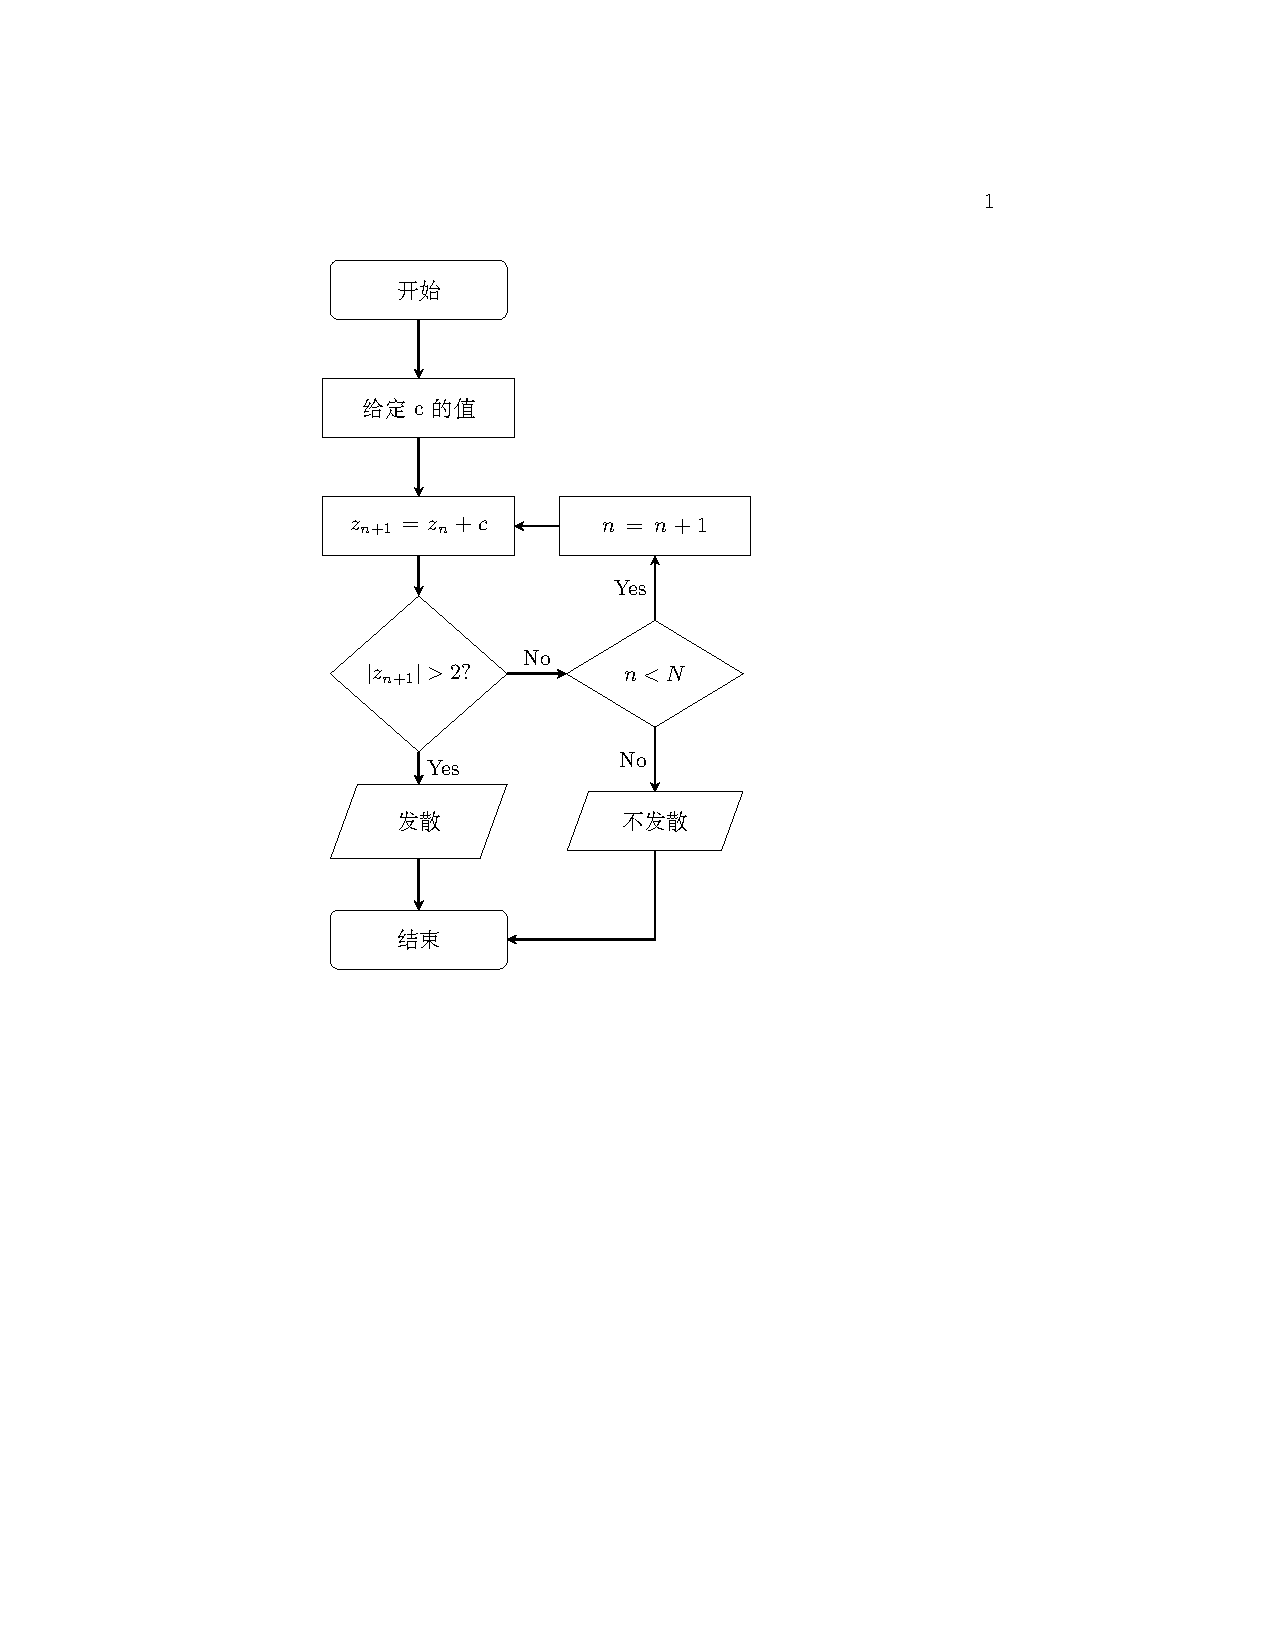
\includegraphics[width=10.5cm]{./page.pdf}

\end{frame}

\section{Julia set 效果图展示}
   \begin{figure}[htbp]
\centering

\subfigure{
\begin{minipage}[t]{0.3\linewidth}
\centering
\includegraphics[width=1.4in]{./photo/-0.80.1560.bmp}

\end{minipage}
}
\subfigure{
\begin{minipage}[t]{0.3\linewidth}
\centering
\includegraphics[width=1.4in]{./photo/-0.70.16.bmp}

\end{minipage}
}

\subfigure{
\begin{minipage}[t]{0.3\linewidth}
\centering
\includegraphics[width=1.4in]{./photo/-0.50.5.bmp}

\end{minipage}
}
\subfigure{
\begin{minipage}[t]{0.3\linewidth}
\centering
\includegraphics[width=1.4in]{./photo/0-0.5.bmp}

\end{minipage}
}

\subfigure{
\begin{minipage}[t]{0.3\linewidth}
\centering
\includegraphics[width=1.4in]{./photo/0.255.bmp}
\end{minipage}
}
\subfigure{
\begin{minipage}[t]{0.3\linewidth}
\centering
\includegraphics[width=1.4in]{./photo/-0.80.1.bmp}

\end{minipage}
}
\end{figure}


\end{document}





